\subsection{Naive Implementation of AES-128}

The naive implementation of our AES-128 algorithm is heavily inspired by the implementation of Rijndael/AES in the book \textit{The Design of Rijndael} \cite{rijndael}. This implementation sets the stage for the structure of all the following subsequent implementations by decomposing into the same conceptual steps as specified in the book, namely; \texttt{SubBytes}, \texttt{ShiftRows}, \texttt{MixColumns}, and \texttt{AddRoundKey}.

In contrast to the more general Rijndael description in the book \cite{rijndael},
our implementation is restricted to the AES-128 variant, and therefore
only considers the case when $N_{b} = 4$ (corresponding to a 128-bit block).

Using the test vectors from the book \cite{rijndael_test_vectors}, we tested not only full end-to-end encryption/decryption, but also the intermediate states before/after each transformation step at each round. Because every transformation step is a separate testable function, we can evaluate these known intermediate states and assert that the output matches the published state for that step.

This makes the implementation closely follow the "textbook" structure and our unit testing approach also allows us to isolate regressions by having fine-grained tests that fail as soon as a single transformation deviates, rather than only detecting mismatches at the final ciphertext.

\subsubsection{Encryption}

Before the encryption process, a set of key schedules are pre-computed and passed to the encryption algorithm.

The encryption process begins by mapping a 16-byte plaintext array to a $4 \times 4$ matrix. This matrix is what we have aptly named the "state" and is what we will perform the operations upon. Each byte is arranged in the following form:

\begin{figure}[H]
    \begin{align*}
        \begin{bmatrix}
            p_{0} & p_{4} & p_{8} & p_{12} \\
            p_{1} & p_{5} & p_{9} & p_{13} \\
            p_{2} & p_{6} & p_{10} & p_{14} \\
            p_{3} & p_{7} & p_{11} & p_{15}
        \end{bmatrix}
    \end{align*}
    \caption{16-byte block transformed to a $4 \times 4$ matrix.}
    \label{fig:state_matrix}
\end{figure}

\noindent
The core of the encryption process is broken into four distinct operations:

\begin{itemize}
    \item \textbf{add\_round\_key}: Using the round as the index for the pre-computed key schedules, the extracted 16-byte "round key" is transformed into a matrix just as we did with the state. Then a bitwise XOR is applied between the state and this "round key" matrix and the state is then updated with this new transformation.

    \begin{figure}[H]
        \centering
        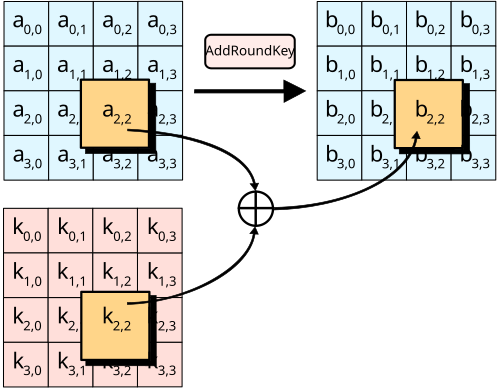
\includegraphics[width=0.7\textwidth]{images/add_round_key.png}
        \caption{AddRoundKey transformation \cite{add_round_key_image}.}
        \label{fig:add_round_key}
    \end{figure}

    \item \texttt{sub\_bytes}: This is a simple substitution step in which each byte in the matrix state is replaced by a corresponding byte from the fixed S-box lookup table.

    \begin{figure}[H]
        \centering
        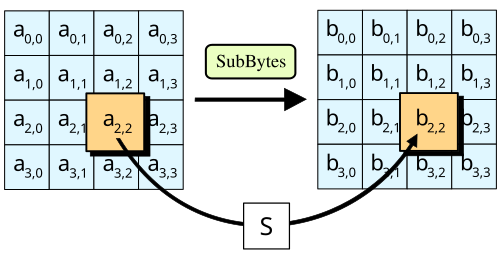
\includegraphics[width=0.7\textwidth]{images/sub_bytes.png}
        \caption{SubBytes transformation \cite{sub_bytes_image}.}
        \label{fig:sub_bytes}
    \end{figure}

    \item \textbf{shift\_rows}: This step shifts the bytes in the last three rows of the state by varying offsets; the first row remains unchanged, while the second, third, and fourth rows are shifted to the left by one, two, and three bytes, respectively.

    \begin{figure}[H]
        \centering
        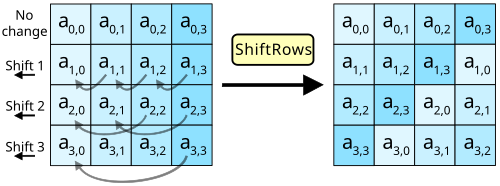
\includegraphics[width=0.7\textwidth]{images/shift_rows.png}
        \caption{ShiftRows transformation \cite{shift_rows_image}.}
        \label{fig:shift_rows}
    \end{figure}

    \item \textbf{mix\_columns}: This step is where much of the diffusion of the ciphertext takes place. It takes each column of the matrix state and treats it as a polynomial over the Galois Field $\text{GF}(2^8)$ and multiplies by a fixed matrix.

    \begin{figure}[H]
        \centering
        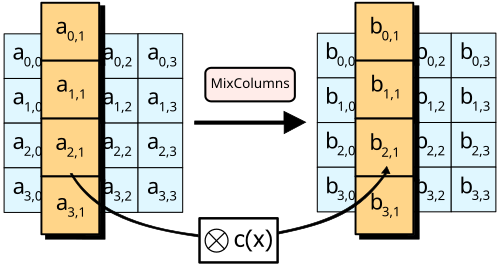
\includegraphics[width=0.7\textwidth]{images/mix_columns.png}
        \caption{MixColumns transformation \cite{mix_columns_image}.}
        \label{fig:mix_columns}
    \end{figure}

\end{itemize}

\subsubsection{Encryption}

We start with round 0, which simply applies an initial \texttt{add\_round\_key} operation.

Following the initial key addition, the state undergoes nine identical ordinary rounds. Each round applies the four transformations mentioned above in the sequence shown in \ref{fig:encryption_round}.

\begin{figure}[H]
    \centering
    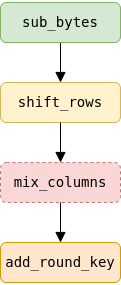
\includegraphics[height=0.4\textwidth]{images/encryption_round.png}
    \caption{Decryption round. \texttt{mix\_columns} is omitted in the last round.}
    \label{fig:encryption_round}
\end{figure}

The tenth and final round is slightly different; it applies the normal operations, but explicitly omits the \texttt{mix\_columns} step. Finally, the resulting state matrix is flattened back into a 1-dimensional 16-byte ciphertext array.

\subsubsection{Decryption}

Similar to the encryption process, the key schedules are pre-computed and the 16-byte ciphertext is transformed into a $4 \times 4$ state matrix.

The decryption process undoes the encryption by applying the inverse of each transformation in reverse order beginning with the initial \texttt{add\_round\_key}, using the final round key of the pre-computed key schedules, followed by \texttt{inverse\_sub\_bytes} and \texttt{inverse\_shift\_rows}.

The state then undergoes nine inverse rounds. Because the operations are applied in reverse, each round consists of the sequence shown in \ref{fig:decryption_round}.

\begin{figure}[H]
    \centering
    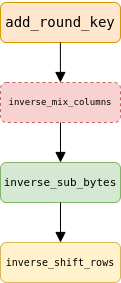
\includegraphics[height=0.4\textwidth]{images/decryption_round.png}
    \caption{Decryption round. \texttt{inverse\_mix\_columns} is omitted in the first round.}
    \label{fig:decryption_round}
\end{figure}

Similar to the encryption operation flow, the \texttt{inverse\_mix\_columns} step utilizes matrix multiplication over $\text{GF}(2^8)$, but with a different set of fixed polynomial constants.

Finally, a concluding \texttt{add\_round\_key} (much like round 0 in the encryption process) is applied using the very first key from the key schedule, and then the decrypted state is flattened back into the 16-byte plaintext array. Thus, fully reversing the encryption process.

\subsection{Optimized Implementation of AES-128}

This section describes the architectural and logic level changes made when transitioning from the naive AES version to an optimized version using a flattened state representation and loop unrolling. The goal of these changes was to reduce instruction overhead and improve execution efficiency.

The first optimization involved flattening the AES state from a two dimensional array (uint8\_t state[4][4]) into a one dimensional array (uint8\_t state[16]). Although multidimensional arrays are already stored linearly in memory, the flat representation simplifies indexing and produces more predictable memory access patterns in performance critical code. Since modern processors load memory in cache line sized blocks (typically 64 bytes), the entire 16 byte AES state fits within a single cache line, improving spatial locality and enabling more efficient register usage and compiler optimization during round transformations.

The second optimization involved manually unrolling loops in the AES operation functions. In the naive implementation, these operations relied on nested loops that introduced additional instructions for counter updates, comparisons, and conditional branching. Loop unrolling exposes more independent instructions to the processor, improving instruction scheduling, register reuse, and instruction level parallelism, which increases overall efficiency.

The third optimization targeted the \texttt{mix\_columns} and \texttt{inv\_mix\_columns} transformations. In the naive implementation, the \texttt{mix\_columns} transformation used a general finite field multiplication routine based on logarithmic lookup tables, which introduced additional memory accesses and control overhead. In the optimized version, these operations were replaced with fixed combinations of shift and XOR operations using the \texttt{xtime} primitive. Using this \texttt{xtime} operation, multiplication by 0x02 is implemented and multiplication by other constants is constructed from combinations of this primitive and XOR operations based on the tables in \ref{fig:mix_columns_tables}. This reduces memory usage and instruction overhead, allowing the transformation to execute more efficiently on the CPU.

These changes transform the implementation from a readable version into a performance oriented version that reduces overhead, and increases instruction level parallelism, which improve the overall efficiency.

\begin{figure}[H]
    \centering
    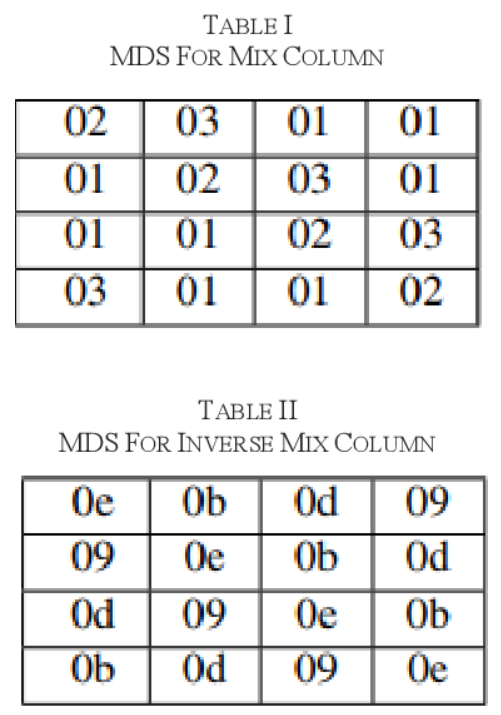
\includegraphics[height=0.4\textwidth]{docs/report/images/mix_columns_tables.png}
    \caption{Tables used for calculating the next state in mix\_columns and inv\_mix\_columns \cite{mix_columns_tables_image}.}
    \label{fig:mix_columns_tables}
\end{figure}

\subsubsection{Encryption/Decryption}

Encryption and decryption works the same as described before in the naive version apart from the flattened state.

\subsection{Implementation of AES-128 using T-tables}

The T-tables approach for AES is a software optimization that merges SubBytes, ShiftRows and MixColumns transformations into precomputed lookup tables. Each lookup table contains 256 entries, with each entry representing the combined result of all transformations applied to a single byte in a specific column position. The first table is created by combining these steps for one byte position and the other three tables are generated by rotating the bytes of the first table to match the remaining column positions. By combining these steps into single byte entries, each byte of the state can be transformed using a single table lookup and XOR operations. This significantly reduces the computational time compared to preforming the transformations separately, improving performance and speed at the cost of additional memory for storing the tables.


\subsubsection{Encryption}

For encryption, four T-tables T0-T3 are used to represent the combined SubBytes, ShiftRows and MixColumns operations for each byte position in a 32-bit column. For each state, the four bytes are used as indices into the corresponding T-tables and outputs are XORed together. The final step is XORing it with RoundKey. By combining multiple transformations into a single table lookup per byte, each round of encryption requires only four table look ups per column and XOR operations.


\subsubsection{Decryption}

For decryption, separate four T-tables TD0-TD3 are constructed to combine the inverse transformation (Inverse SubBytes, ShiftRows and MixColumns). Each byte of a ciphertext column is used to index the corresponding inverse table, and the results are XORed together with the round key. This allows the inverse round transformations to be performed efficiently in a single step per byte.

\subsection{Implementation of AES-128 using NI instructions}

Up until now, AES has been implemented at the software level as algorithms written directly in C code. However, Intel introduced an extension instruction set for their x86 architecture known as Advanced Encryption Standard New Instructions (AES-NI). AES-NI allows complex AES operations to be executed directly on the hardware, significantly accelerating the encryption and decryption processes, while also mitigating the risk of side-channel attacks by eliminating the need for software-based lookup tables.

In C, these hardware instructions are accessed through intrinsics from the \texttt{\textless wmmintrin.h\textgreater} header. This interface allows access to several instructions and types without the need to write the underlying assembly. The interface provides a convenient type \texttt{\_\_m128i}, which represents a 128-bit register, so an entire AES block can be loaded into a single CPU register and processed there rather than repeatedly reading and writing individual bytes in memory.

A major consequence of using AES-NI is that several helper functions from the other implementations, such as \texttt{add\_round\_key}, \texttt{mix\_columns}, \texttt{shift\_rows}, \texttt{inverse\_mix\_columns} and \texttt{inverse\_shift\_rows}, are no longer needed in the encryption/decryption processes, since their work is effectively absorbed into the CPU instructions themselves.

\subsubsection{Encryption}

First the plaintext block and the first round key are loaded into hardware registers with \texttt{\_mm\_loadu\_si128}, and the initial key addition is performed with \texttt{\_mm\_xor\_si128}. Next, the nine main rounds are handled by \texttt{\_mm\_aesenc\_si128}, which applies the standard round transformation in hardware, and the final round is performed by \texttt{\_mm\_aesenclast\_si128} - a separate instruction because the last AES round, as mentioned before, omits the mix columns step.

Once the computation is finished, the resulting ciphertext is copied back to memory using \texttt{\_mm\_storeu\_si128}.

\subsubsection{Decryption}

As with encryption, decryption follows the same overall idea, but using the inverse hardware instructions. The ciphertext is loaded into a register, combined with the last round key, and then processed through \texttt{\_mm\_aesdec\_si128} for the intermediate rounds. Finally, the special \texttt{\_mm\_aesdeclast\_si128} instruction is used for the last round to omit the inverse mix columns step. Before those intermediate decryption rounds, each round key is transformed with \texttt{\_mm\_aesimc\_si128}, because the decryption instructions expect the keys in a form adapted to the inverse round structure.

Similar to the encryption process, once the computation is finished, the resulting plaintext is copied back to memory using \texttt{\_mm\_storeu\_si128}.
